\section{Architecture générale}

Afin de pouvoir tirer profit de l’infrastructure de stockage distribué offerte par Ceph, de nombreuses interfaces ont étés développées (cf figure \ref{chap2:stack}) afin d'offrir un large panel de possibilités aux utilisateurs. Ces interfaces sont des points d'accès au même composant central assurant la gestion des données distribuées : \textbf{RADOS}\footnote{RADOS signifie Reliable Autonomic Distributed Object Store, littéralement Stockage d'objets fiable, automatique et distribué.}. Cet élément est crucial et gère toute la logique liée à la distribution et la réplication des données. De ce fait, une partie lui sera dédiée plus tard dans le présent rapport. 

Nous présentons d'abord les différents éléments composants Ceph, puis détaillons en profondeur les concepts.

\begin{figure}[h]
    \centering
    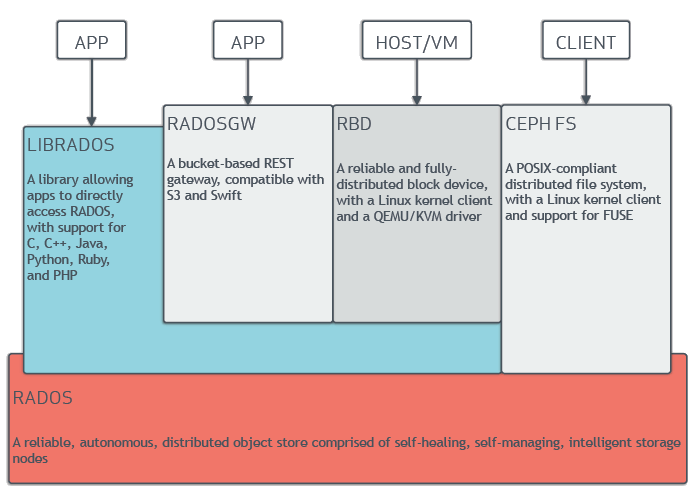
\includegraphics[scale=0.5]{./images/stack.png}
    \caption{Aperçu de l'architecture générale de Ceph}
    \label{chap2:stack}
\end{figure}

\subsection{Librados}
Afin de pouvoir construire des applications basée sur RADOS, la bibliothèque \textbf{Librados} a été développée dans le but de pouvoir interagir au plus bas niveau avec le cluster Ceph. Cette bibliothèque écrite en langage C permet en particulier d'accéder directement et de façon concurrente au cluster. Des bilbliothèques similaires ont étés développées dans d'autres langages comme Python, Java et C++. 

L'utilisation de librados pour communiquer directement avec RADOS améliore drastiquement les performances des applications tout en leur offrant un maximum de fiabilité et de flexibilité.

\subsection{Interfaces offertes par Ceph}

Outre l'interface native de Ceph, il existe d'autres modes d'accès  à RADOS. Avant de détailler ces interfaces, il est important de signaler qu'il est possible d'utiliser \textbf{plusieurs interfaces} pour un même cluster, il n'est par exemple pas nécessaire de configurer trois clusters différents pour trois interface.

\paragraph{Rados block device (RBD)}

Ce dispositif découpe une image de \textbf{périphérique bloc} sur plusieurs objets dans le cluster de stockage Ceph, où chaque objet est mappé sur un groupe de placement\footnote{Nous y reviendrons, mais disons simplement qu'il s'agit d'une entité permettant d'agréger des objets.} et distribué.

Ces techniques se révèlent être des options intéressantes pour la virtualisation et le cloud computing. Dans les scénarii basés sur des machines virtuelles, il est de mise de déployer en général ce dispositif avec le pilote de stockage réseau $rbd$ dans QEMU\footnote{QEMU est un logiciel libre de machine virtuelle.} / KVM\footnote{KVM est un hyperviseur de type I sous Linux.}, où l'ordinateur hôte utilise la librairie librbd \footnote{Fournit un accès en forme de fichier aux images RBD.} pour fournir un service de périphérique bloc au client. 

\paragraph{RADOSGW}
RADOSGW (RADOS Getaway) est une interface de \textbf{stockage d'objets} construite au dessus de librados pour fournir aux applications une passerelle RESTful \footnote{API Restful : interface de programmation d'application qui fait appel à des requêtes HTTP pour obtenir (GET), placer (PUT), publier (POST) et supprimer (DELETE) des données.} aux clusters de stockage Ceph. Deux interfaces sont possibles:

\begin{itemize}
\item S3 - compatible : fournit une fonctionnalité de stockage d'objet avec une interface compatible avec un grand sous-ensemble de l'API Amazon S3 \footnote{Amazon S3 : site d'hébergement de fichiers offert par Amazon Web Services.} RESTful.
\item Swift-compatible : fournit une fonctionnalité de stockage d'objet avec une interface compatible avec un grand sous-ensemble de l'API OpenStack Swift \footnote{Système de stockage de données d'OpenStack.}.
\end{itemize}

L'utilisation couplée de ces deux API est possible. Par exemple, vous pouvez écrire des données à l'aide de l'API compatible S3 avec une application, puis lire des données à l'aide de l'API Swift compatible avec une autre application.

\paragraph{CephFS}

Le \textbf{système de fichiers} Ceph (CephFS) est un système de fichiers respectant la norme POSIX qui utilise un cluster de stockage Ceph pour stocker les fichiers. Les fichiers CephFS sont mappés sur des objets que Ceph stocke dans le cluster de stockage. Les clients Ceph ont le choix de monter un système de fichiers CephFS comme un objet kernel ou un système de fichiers dans un espace utilisateur (FUSE).

Ce service inclut le serveur de métadonnées Ceph (MDS) déployé avec le cluster Ceph Storage. L'objectif du MDS est de stocker toutes les métadonnées du système de fichiers (répertoires, propriété des fichiers, modes d'accès, etc.) dans les serveurs de Ceph haute disponibilité où les métadonnées se trouvent dans la mémoire. L'idée derrière le MDS est que les opérations simples du système de fichiers comme l'affichage du contenu d'un répertoire ou la modification d'un répertoire (ls, cd) ne doivent pas surcharger inutilement les démons Ceph OSD. Ainsi, la séparation des métadonnées des données signifie que le système de fichiers Ceph peut fournir des services performants sans surcharger le cluster de stockage Ceph.
